\usepackage{amsmath,amsfonts,amssymb,amsthm,mathtools} 
\usepackage{icomma} 
\usepackage{wasysym}
\documentclass[a4paper,12pt]{article} % тип документа
\usepackage[left=2.5cm,right=2.5cm,
    top=2cm,bottom=2cm,bindingoffset=0cm]{geometry}
\usepackage{multirow} 

\usepackage{indentfirst}
\usepackage{floatrow,graphicx,calc}
\usepackage{wrapfig}
\usepackage{xcolor}
\usepackage{hyperref}
\definecolor{linkcolor}{HTML}{799B03} % цвет ссылок
\definecolor{urlcolor}{HTML}{799B03} % цвет гиперссылок

\hypersetup{pdfstartview=FitH,  linkcolor=linkcolor,urlcolor=urlcolor, colorlinks=true}

\usepackage{graphicx}  
\graphicspath{{images/}{images2/}} 
\setlength\fboxsep{3pt} 
\setlength\fboxrule{1pt} 
\usepackage{wrapfig} 

\DeclareFloatSeparators{mysep}{\hspace{1cm}}

\usepackage{hyperref}
\usepackage[rgb]{xcolor}
\hypersetup{				
    colorlinks=true,       	
	urlcolor=blue          
}

\usepackage[T2A]{fontenc}			
\usepackage[utf8]{inputenc}			
\usepackage[english,russian]{babel}	

\usepackage{amsmath,amsfonts,amssymb,amsthm,mathtools}

\usepackage{amsmath,amsfonts,amssymb,amsthm,mathtools} 
\usepackage{icomma} 
\usepackage{wasysym}

\begin{document}
\begin{center}
	\footnotesize{ФЕДЕРАЛЬНОЕ ГОСУДАРСТВЕННОЕ АВТОНОМНОЕ ОБРАЗОВАТЕЛЬНОЕ 			УЧРЕЖДЕНИЕ ВЫСШЕГО ОБРАЗОВАНИЯ}\\
	\footnotesize{МОСКОВСКИЙ ФИЗИКО-ТЕХНИЧЕСКИЙ ИНСТИТУТ\\(НАЦИОНАЛЬНЫЙ 			ИССЛЕДОВАТЕЛЬСКИЙ УНИВЕРСИТЕТ)}\\
	\footnotesize{ФАКУЛЬТЕТ ОБЩЕЙ И ПРИКЛАДНОЙ ФИЗИКИ\\}
	\hfill \break
	\hfill \break
	\hfill \break
	\hfill \break
\end{center}


\begin{figure*}[h]
    \centering
    \includegraphics*[width=10cm,height=7cm,keepaspectratio]{mipt.png}
    \label{mipt.png}
\end{figure*}


\begin{center}   
    \hfill \break
	\hfill \break
	\hfill \break
	\hfill \break
	\large{Отчёт о выполнении лабораторной работы № 3.7.3\\\textbf{ДЛИННЫЕ ЛИНИИ}}\\
	\hfill \break
	\hfill \break
	\hfill \break
	\hfill \break
	\begin{flushright}
		Легких Никита \\ Б05-301
	\end{flushright}
	\hfill \break
	\hfill \break
	\hfill \break
\end{center}
\hfill \break


\begin{center}
	Долгопрудный, 2024 г.
\end{center}
\thispagestyle{empty}
\newpage
\pagenumbering{gobble} 

\begin{flushleft}
\section*{В работе используются:}
 
Осциллограф АКТАКОМ ADS-6142H; генератора АКИП 3420/1; бухта с
коаксиальным кабелем pk 50-4-11; схематический блок "модель длинной линии"; магазин
сопротивления Р33, соединительные провода.

\end{flushleft}

\section*{Теоретическая справка}
Рассмотрим элемент dx длинного коаксиального кабеля:
\begin{figure}[h]
	\centering
	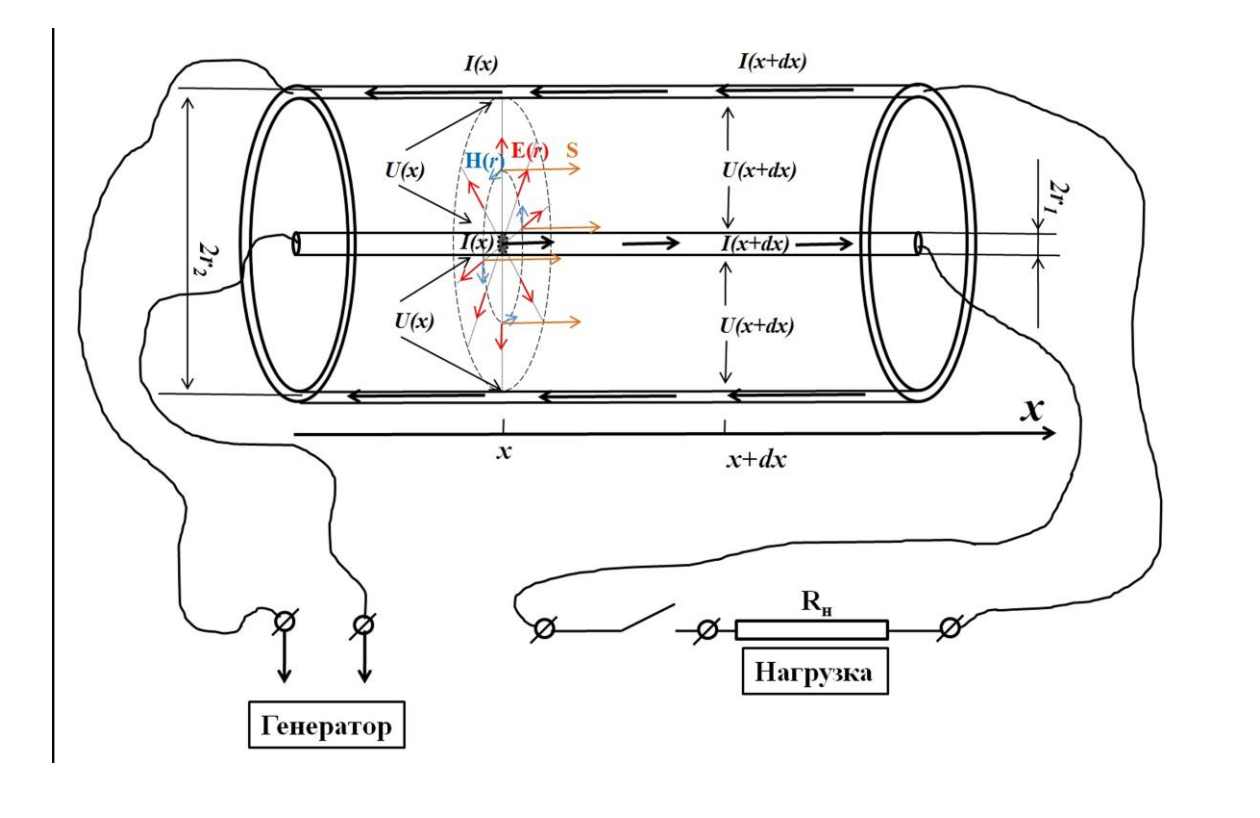
\includegraphics[scale=0.5]{dx.png}
	\caption{Схематическое изображение элемента dx длинного коаксиального кабеля.} 
\end{figure}

\begin{enumerate}
    \item Удельная (погонная) индуктивность единицы длины такого кабеля: 
    \begin{equation}
    L_x =  \mu ln(r_2/r_1)
\end{equation}
    \item Удельная (погонная) ёмкость единицы длины кабеля:
    \begin{equation}
    C_x = \frac{\varepsilon}{2ln(r_2/r_1)}
\end{equation}
    \item Когда по кабелю передаётся сигнал, в его центральной жиле и внешней оболочке возникают взаимно противоположные токи I(x), а также электрическое напряжение U(x) между внешним и внутренним проводниками. Изменение напряжения на концах элемента dx вызваны возникновением ЭДС индукции и
падением напряжения в результате омического сопротивления проводников: 
\begin{equation}
    U(x+dx) - U(x) = - \frac{L_x dx}{c^2} \frac{\partial I}{\partial t} - R_x dxI,
\end{equation} 
где погонное сопротивление:
\begin{equation}
    R_x = \frac{1}{\sigma \cdot S}
\end{equation} 
$\sigma$ - удельная проводимость материала проводников, S - площадь их поперечного
сечения.

\item Изменение силы тока вызвано тем, что некоторая часть электрического заряда q как бы "перетекает на "обкладки" конденсатора, роль которых играют проводники коаксиального
кабеля: 
\begin{equation}
    I(x+dx) - I(x) = - \frac{\partial q}{\partial t},
\end{equation} 
q = $C_x dx U$ .
\item После представления уравнений (3) и (5) в виде системы, описывающей распространение сигнала
вдоль длинной линии, и нахождения ее решений было получено волновое уравнение в каноническом виде:
\begin{equation}
   \frac{\partial^2 U}{\partial t^2} - V^2_\text{ф} \frac{\partial^2 U}{\partial x^2} + \gamma \frac{\partial U}{\partial t} = 0,
\end{equation} 
Фазовая скорость
\begin{equation}
   V_\text{ф} = \frac{c}{\sqrt{L_x C_x}}
\end{equation} 
Декремент затухания
\begin{equation}
   \gamma = R_x C_x V_\text{ф}^2
\end{equation}


Можно заметить, что фазовая скорость имеет тот же вид, как и скорость распространения обычных электромагнитных
волн в некоторой среде с диэлектрической проницаемостью $\varepsilon$ и магнитной
восприимчивостью $\mu$: 
\begin{equation}
   V_\text{ф} = \frac{c}{\sqrt{\varepsilon \mu}}
\end{equation}
\item После установления характера изменения силы тока в
длинной линии, видно, что отношение силы тока и напряжения в длинной линии не зависят от времени и координаты. Это отношение называют волновым сопротивлением
(импедансом) и в пределе малых затуханий он выражается:
\begin{equation}
  Z(\omega, k) = \frac{1}{c}\sqrt{\frac{L_x}{C_x}}
\end{equation}
\item Если в конце такую длинную линию замкнуть на сопротивление
$R_0 = Z(\omega, k)$, то бегущая вдоль длинной линии волна "будет воспринимать" нагрузку как бесконечное
продолжение этой длинной линии (отражённой волны не возникает). Во всех остальных
случаях, возникает отражённая волна,
описываемая выражением (сравни с (13)):
\begin{equation}
  U(x,t) = U_0 e^{- iwt}e^{-(\alpha +ik)x}
\end{equation}
Амплитуда колебаний на согласованной нагрузке (в конце длинной линии):
\begin{equation}
 U_H = U_0 e^{-\alpha t}
\end{equation}
Набег фазы сигнала на выходе (в конце длинной линии) относительно входного сигнала
(вначале длинной линии)
\begin{equation}
  \Delta \phi = kl
\end{equation}
Из (11) и (12) легко экспериментально определить декремент затухания $\alpha$ и волновое
число k для различных $\omega$:
\begin{equation}
  \alpha(\omega) = \frac{1}{l}ln(\frac{U_H}{U_0})
\end{equation}
\begin{equation}
  k(\omega) = \frac{\Delta \phi}{l}
\end{equation}
\end{enumerate}

\section*{Экспериментальная установка}

Для проведения эксперимента была собрана схема согласно рис.2.

\begin{figure}[h]
	\centering
	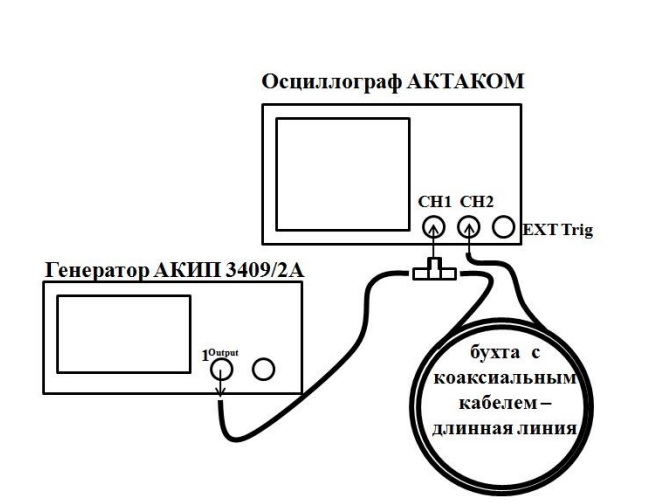
\includegraphics[scale=0.7]{cx.png}
	\caption{ Схема установки для наблюдения
распространения сигналов вдоль длинной линии.} 
\end{figure}
Для этого:
а) один конец коаксиального кабеля с
помощью "тройника" был подключен к выходу
"1" генератора и ко входу CH1 осциллографа
(для соединения тройника с генератором
использовался короткий коаксиальный кабель;
тройник напрямую подключался к
осциллографу, чтобы сдвиг фазы сигнала на
входе в осциллограф и в начале "длинной
линии" был минимален);
б) второй конец кабеля "длинной
линии" был подключен ко входу CH2
осциллографа.

\section*{Ход работы}
\subsection*{I. Оценка фазовой и групповой скорости}
\textbf{Синусоидальный сигнал (согласованная линия):}
\\
Длинная линия была нагружена согласованной нагрузкой (выставлено сопротивление 50 Ом) 
\begin{enumerate}

\item Меняя частоту выходного сигнала генератора в пределах от 1 МГц до 30 МГц и подбирая необходимые параметры вертикальной и горизонтальной развёрток
осциллографа, были качественно наблюдаемы изменения сигнала (сдвиг фазы и
амплитуда) в начале и в конце (на согласованной нагрузке) в длинной линии.

\item Экспериментально определенные резонансные частоты (случай, когда "нули" или локальные экстремумы функций сигналов в начале и конце длинной линии совпадают) имели значения: $\nu =  $ 2, 6, 10, 14, 18, 22, 26 МГц\\
Резонансные частоты соответствуют ситуации, когда сдвиг фаз между сигналом на входе и выходе длинной линии кратен 2$\pi$.
\item При помощи анализа набора резонансных частот оценка величины фазовой скорости составила $ V_\text{ф} = (\omega_2 - \omega_1) \cdot l = 4 \cdot 10^6 \cdot 50,1 = 2 \cdot 10^8  $ (м/с).
таким образом был сделан вывод об отсутствии дисперсии в данном диапазоне частот.
\end{enumerate}
\paragraph{}
\textbf{Синусоидальный сигнал (линия без нагрузки):}\\
Было выставлено сопротивление 1 МОм), что моделирует незамкнутый выход
(отсутствие нагрузки) в конце длинной линии.
\begin{enumerate}
\item Аналогично 1 пункту при согласованной линии
\item  Экспериментально определенные резонансные частоты : $ \nu =  $ 2, 6, 10, 14, 18, 22, 26 МГц
\item Величина фазовой скорости $ V_\text{ф} = 2 \cdot 10^8  $ (м/с), что свидетельствовало об отсутствии дисперсии в данном диапазоне частот.
\end{enumerate}

\textbf{Прямоугольные импульсы (согласованная линия):}\\
Была выставлена величина сопротивления 50 Ом, что соответствовало согласованной нагрузке в
конце длинной линии.
\begin{enumerate}
\item Меняя частоту и длительность импульсов во всех допустимых пределах генератора и подбирая необходимые параметры вертикальной и горизонтальной развёрток
осциллографа были качественно наблюдаемы изменения сигнала в начале и в конце (на
согласованной нагрузке) в длинной линии.
\item Меняя частоты повторения импульсов от 1 МГц до 20 МГц были определены резонансные частоты: $\nu =  $ 4, 8, 12, 16, 20 МГц. Таким образом был сделан вывод об отсутствии дисперсии в данном диапазоне частот.
\end{enumerate}

\textbf{Прямоугольные импульсы (линия без нагрузки):} \\
Было выставлено сопротивление 1 МОм, что моделирует незамкнутый выход (отсутствие нагрузки) в конце длинной линии.
\begin{enumerate}
\item Аналогично пункту 1 для согласованных линий.
\item Резонансные частоты $\nu =  $ 4, 8, 12, 16, 20 МГц, следовательно был сделан вывод об отсутствии дисперсии в данном диапазоне частот.
\end{enumerate}

\subsection*{II. Амплитудно-частотная и фазово-частотная характеристики}
Было выставлено сопротивление 50 Ом, что соответствует согласованной нагрузке в
конце длинной линии, и выбран синусоидальный сигнал "Синус".\\
Была установлена частота сигнала около 2-5 МГц и амплитуда сигнала 4 В \\
Фазу и смещение приравняли к нулю, нагрузку установили равной 50 Ом.
\paragraph{}
Меняя частоту выходного сигнала генератора в пределах от 1 МГц до 40 МГц, были сняты АЧХ и ФЧХ длинной линии.


\begin{table}[h]
	\centering
	\begin{tabular}{|c|c|c|c|c|c|c|c|}
	    \hline
		$\nu$, МГц& $U_1$, B& $U_2$, B & $\alpha \cdot 10^5 $, B&  Ф$_1$& Ф$_2$& Ф$_2$ - Ф$_1$ &$k*10^5$  \\ \hline
		2& 52,8 & 50,0 & 1,088 &-176,4 & 176,4 &187,2 &65,2\\ \hline
		4& 52,8 & 48,4 & 1,737&5,7 & -5,7 & 371,4& 129,3 \\ \hline
            6& 52,8 & 46,8 &2,408&-174 & 174 & 552&192,2 \\ \hline
            8& 52,8 & 45,6 & 2,926&8,46 & -8,46 & 736,92 & 256,6\\ \hline
            10& 52,8 & 45,2 & 3,102&-169,2 & 169,2 & 921,6 & 320,9  \\ \hline
            12& 53,2 & 44,0 & 3,79&8,64 & -10,08 & 1098,72 & 382,6  \\ \hline
            14& 52,8 & 43,6 & 3,821&-168,7 & 171,4&  1279,9 & 445,7  \\ \hline
             \end{tabular}
    \end{table}

    \begin{table}[h]
	\centering
        \caption{АЧХ и ФЧХ}  \label{decr}
	\begin{tabular}{|c|c|c|c|c|c|c|c|}
	    \hline
		$\nu$, МГц& $U_1$, B& $U_2$, B & $\alpha \cdot 10^5 $ &  Ф$_1$& Ф$_2$& Ф$_1$ - Ф$_1$ & $k*10^5$  \\ \hline
            16& 53,2 & 42,8 & 4,342&11,52 & -8,64 & 1460,16& 508,4 \\ \hline
            18& 53,2 & 42,4 & 4,529&-172,282 & 168,532& 1639,186 & 570,8  \\ \hline
            20& 53,2 & 42,0 & 4,718&14,4 & -14,4 & 1828,8 & 636,8   \\ \hline
            22& 52,99 & 41,30 & 4,975& -173,14 & 174,19& 1992,67 &693,8 \\ \hline
            24& 52,89 & 40,58 & 5,288&-5,76 & 6,912 & 2172,672 &756,5 \\ \hline
            26& 52,52 & 39,77 & 5,551&-172,825 & 172,201 & 2354,974  & 820 \\ \hline
            28& 52,55 & 38,96 & 5,973&8,067 & -7,552 & 2535,619 &882,9\\ \hline
            30& 52,23 & 38,51 & 6,083&-170,015 & 170,555 & 2715,43 &945,5  \\ \hline
            32& 52,74 & 38,14 & 6,469&6,912 & -7,448 & 2894,36 &1007,8 \\ \hline
            34& 52,77 & 37,36 & 6,893&-171,429 & 173,878 & 3074,693 & 1070,6\\ \hline
            36& 52,74 & 36,43& 7,385&7,70 & -7,70 & 3255 &1133,5 \\ \hline
            38& 52,71 & 35,79 & 7,727&-173,982 & 172,340 & 3433,678 & 1195,6\\ \hline
            40& 52,35 & 35,03 & 8,019&8,640& -8,640 & 3617,28 &1259,5 \\ \hline
            
	\end{tabular}
\end{table}


\section*{Обработка результатов}
\subsection*{Определение параметров коаксиального кабеля.}
При помощи построения зависимости
\[y_1 = \frac{L_x C_x}{c^2}x_1, \;\;\; \;\;\;\; \;\;\;\;\; y_1 = k(\omega)^2 - \alpha(\omega)^2 \;\;\; x_1 = \omega^2\]


\begin{figure}[h]
	\centering
	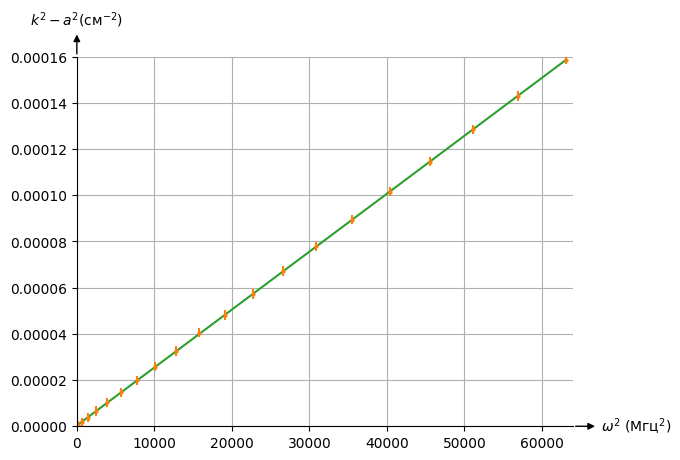
\includegraphics[scale=0.7]{image1.png}
	\caption{ Зависимость $y_1(x_1)$} 
\end{figure}



Было определено значение $L_x C_x$ = $2,5075 \cdot 10^{-17} $ $\frac{\text{Ф} \cdot \text{Гн}}{\text{м}^2}$ \\
Также, зная волновое сопротивление коаксиального кабеля (согласованную нагрузку) и с учётом формулы (10) были определены погонные характеристики кабеля:
\[L_x = 0,250 \pm 0,005 \frac{\text{мкГ}}{\text{м}}\;\;\;\;\;\;\; C_x = 100 \pm 3 \frac{\text{пФ}}{\text{м}} \]

\textbf{Определение удельной проводимости проводников.}
\paragraph{}
Метод А.
\paragraph{}
Имеем формулу:
\[\alpha(\omega) = \frac{1}{l}ln(\frac{U_0}{U_H}) = R_x \frac{V_\text{ф}}{2}C_x\]

Если взять удельную проводимость для меди и подставить в известное выражение для
характерной толщины скин-слоя:
\[\delta = \frac{c}{2\pi \sqrt{\nu \sigma}}\]
то окажется, что даже при минимальной частоте 1 МГц эта толщина будет равна около 65 мкм, что примерно в десять раз меньше радиуса центрального проводника (диаметр
центральной жилы равен d = 1,37 мм). При больших частотах характерная толщина скинслоя ещё меньше. Поэтому для упрощения будем предполагать, что весь ток сосредоточен
в приповерхностном слое и потери, связанные с джоулевым нагревом описываются
следующим выражением:
\[dN = \frac{(dU)^2}{dR} \;\;\;\;\;\;\; dR = \frac{dx}{\sigma \cdot \pi d} \cdot \frac{2}{\delta}\]
с учётом выражения для характерной толщины скин-слоя:
\[R_x = \frac{4\sqrt{\nu}}{\sqrt{\sigma}\cdot c \cdot d}\]
Таким образом, получается зависимость:
\[y_2 = \frac{4}{\sqrt{\sigma} \cdot d} C_x \frac{V_\text{ф}}{c}x_2\]
\[y_2 = \alpha(\omega)\;\;\;\;\;\;\;x_2 = \sqrt{\nu}\]


\begin{figure}[h]
	\centering
	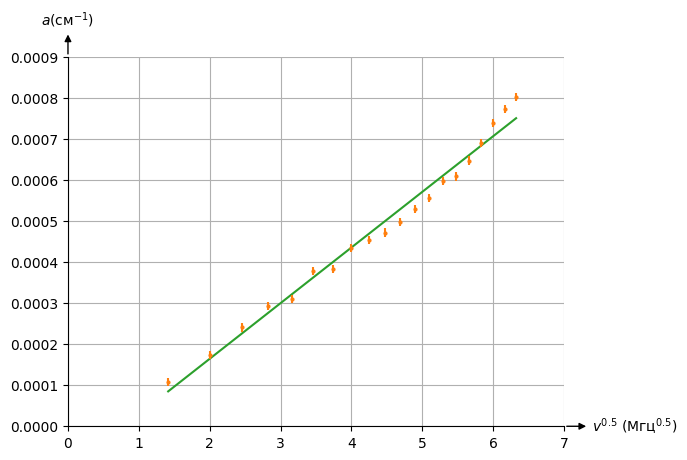
\includegraphics[scale=0.7]{download5.png}
	\caption{ Зависимость $y_2(x_2)$} 
\end{figure}


При помощи построения зависимости декремента затухания $y_2$ от корня частоты гармонического сигнала $x_2$, по углу наклона
прямой была определена удельная проводимость
\[\sigma = (\frac{2C_x V_\text{ф}}{c \cdot d \cdot (\Delta y_2/\Delta x_2)})^2 = (\frac{2 \cdot 958 \cdot 2 \cdot 10^{10}}{3 \cdot 10^{10} \cdot 7,8 \cdot 10^{-1} \cdot (1.355 \cdot10^{-4})})^2 = 1,46 \cdot 10^{14} \text{c}^{-1}\]
\newpage
Метод Б.
\paragraph{}
Подставив выражение для $\gamma$ в другие уравнения было получено
\[2\alpha k = \omega R_x C_x\]
Зная амплитуду колебаний и сдвиг фазы в конце длинной линии относительно входного сигнала экспериментально можно определить как $\alpha(\omega)$, так и $k(\omega)$
Таким образом, можно переписать выражение как 
\[y_3 = \frac{4 \pi C_x}{\sqrt{\sigma} \cdot c \cdot d} x_3  \]
\[y_3 = \frac{1}{l}ln(\frac{U_0}{U_H}) \cdot \frac{\Delta \phi}{l}\;\; \;\;\;\;\;\;\;\;\; x_3 = \nu^{3/2}\]

\begin{figure}[H]
	\centering
	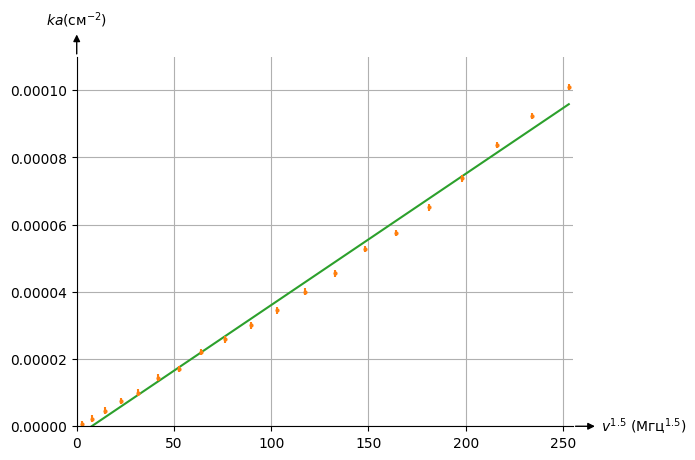
\includegraphics[scale=0.7]{download (6).png}
	\caption{ Зависимость $y_3(x_3)$} 
\end{figure}


Построив полученную зависимость, по наклону была определена удельная проводимость 
\[\sigma = (\frac{4 \pi C_x }{c \cdot d \cdot (\Delta y_3/\Delta x_3)})^2 = 4,95\cdot 10^{17} \text{с}^{-1}\]
Как видим полученные значения удельной проводимости двумя разными методами сходятся с ??? погрешностью, 


\section*{Вывод}
В данной работе было исследованно распространение электрических сигналов вдоль длинной линии.

Для различных сигналов и нагрузок линий были определены фазовые скорости, которые оказались порядка скорости света, что говорит об отсутствии дисперсии в рассматриваемом диапазоне частот. После снятия АЧХ и ФЧХ, при помощи построения различных зависимостей были рассчитаны значения погонных характеристик данной линии. Скорее всего в процессе обработки произошли ошибки, из-за этого значения не сошлись с ожидаемыми

\end{document}
